\documentclass[12pt,]{article}
\usepackage{lmodern}
\usepackage{amssymb,amsmath}
\usepackage{ifxetex,ifluatex}
\usepackage{fixltx2e} % provides \textsubscript
\ifnum 0\ifxetex 1\fi\ifluatex 1\fi=0 % if pdftex
  \usepackage[T1]{fontenc}
  \usepackage[utf8]{inputenc}
  \usepackage{eurosym}
\else % if luatex or xelatex
  \ifxetex
    \usepackage{mathspec}
  \else
    \usepackage{fontspec}
  \fi
  \defaultfontfeatures{Ligatures=TeX,Scale=MatchLowercase}
  \newcommand{\euro}{€}
\fi
% use upquote if available, for straight quotes in verbatim environments
\IfFileExists{upquote.sty}{\usepackage{upquote}}{}
% use microtype if available
\IfFileExists{microtype.sty}{%
\usepackage{microtype}
\UseMicrotypeSet[protrusion]{basicmath} % disable protrusion for tt fonts
}{}
\usepackage[margin=1in]{geometry}
\usepackage{hyperref}
\hypersetup{unicode=true,
            pdftitle={Einkommensverteilung in Österreich},
            pdfauthor={Sarah Gust \& Hubert Weiß},
            pdfkeywords={inequality},
            pdfborder={0 0 0},
            breaklinks=true}
\urlstyle{same}  % don't use monospace font for urls
\usepackage{longtable,booktabs}
\usepackage{graphicx,grffile}
\makeatletter
\def\maxwidth{\ifdim\Gin@nat@width>\linewidth\linewidth\else\Gin@nat@width\fi}
\def\maxheight{\ifdim\Gin@nat@height>\textheight\textheight\else\Gin@nat@height\fi}
\makeatother
% Scale images if necessary, so that they will not overflow the page
% margins by default, and it is still possible to overwrite the defaults
% using explicit options in \includegraphics[width, height, ...]{}
\setkeys{Gin}{width=\maxwidth,height=\maxheight,keepaspectratio}
\IfFileExists{parskip.sty}{%
\usepackage{parskip}
}{% else
\setlength{\parindent}{0pt}
\setlength{\parskip}{6pt plus 2pt minus 1pt}
}
\setlength{\emergencystretch}{3em}  % prevent overfull lines
\providecommand{\tightlist}{%
  \setlength{\itemsep}{0pt}\setlength{\parskip}{0pt}}
\setcounter{secnumdepth}{0}
% Redefines (sub)paragraphs to behave more like sections
\ifx\paragraph\undefined\else
\let\oldparagraph\paragraph
\renewcommand{\paragraph}[1]{\oldparagraph{#1}\mbox{}}
\fi
\ifx\subparagraph\undefined\else
\let\oldsubparagraph\subparagraph
\renewcommand{\subparagraph}[1]{\oldsubparagraph{#1}\mbox{}}
\fi

%%% Use protect on footnotes to avoid problems with footnotes in titles
\let\rmarkdownfootnote\footnote%
\def\footnote{\protect\rmarkdownfootnote}

%%% Change title format to be more compact
\usepackage{titling}

% Create subtitle command for use in maketitle
\newcommand{\subtitle}[1]{
  \posttitle{
    \begin{center}\large#1\end{center}
    }
}

\setlength{\droptitle}{-2em}

  \title{Einkommensverteilung in Österreich}
    \pretitle{\vspace{\droptitle}\centering\huge}
  \posttitle{\par}
  \subtitle{2063 - Ökonomie der Verteilung}
  \author{Sarah Gust \& Hubert Weiß}
    \preauthor{\centering\large\emph}
  \postauthor{\par}
      \predate{\centering\large\emph}
  \postdate{\par}
    \date{04 January, 2019}

% Used for placing figures more precisely
\usepackage{float} 
      \let\origfigure\figure 
      \let\endorigfigure\endfigure
      \renewenvironment{figure}[1][2] {
        \expandafter\origfigure\expandafter[H]
      } {\endorigfigure}

\begin{document}
\maketitle
\begin{abstract}
Dieses Dokument \ldots{}
\end{abstract}

{
\setcounter{tocdepth}{2}
\tableofcontents
}
Zitieren im Text -\textgreater{} Eckige Klammer (Grabka et al. 2016)
Eckige Klammer, cheatsheet, R Markdown Knit geht nicht!!

\newpage

\section{Einleitung}\label{einleitung}

\section{Berechnung allgemeiner
Ungleichheitsindikatoren}\label{berechnung-allgemeiner-ungleichheitsindikatoren}

\subsection{Daten und Berechnungen}\label{daten-und-berechnungen}

Als Datengrundlage verwenden wir die EU-Statistik über Einkommen und
Lebensbedingungen (EU Statistics on Income and Living Conditions --
EU-SILC) von 2005 bis 2017. Zur Berechunung der Ungleichheitsentwicklung
in Deutschland wurden drei verschiedene Einkommenskomponenten
herangezogen. Das vorsteuerliche Faktoreinkommen (Pre-tax factor income)
umfasst Arbeits- und Vermögenseinkommen. Die entsprechenden
Ungleichheitsindikatoren geben wieder, wie hoch die Ungleichheit in
Deutschalnd wäre, gäbe es kein öffentliches Transfersytem. Das Pre-tax
national income erfasst zusätzlich Pensionen und Arbeitslosengeld. Das
nachsteurliche, verfügbare Einkommen (Post-tax disposable income) zeigt,
wie der Staat die Verteilung der verfügbaren Einkommen durch Steuern und
Sozialleistungen beeinflusst. Diese Einkommenskonzepte wurden auf
jeweils zwei unterschiedliche Arten aufgeteilt: 1. Alle Einkommensgrößen
werden in gleichen Anteilen durch alle Haushaltsmitglieder geteilt
(equal sharing of resources within household) und 2. die
personenbezogenen Einkommensgrößen bleiben den entsprechenden Personen
zugeordnet, die Haushalsgrößen werden durch Haushaltsmitglieder geteilt,
die älter als 19 Jahre sind (partial sharing of resources).
Einkommenskomponenten unter null wurden von der Berechnung der
Indikatoren ausgeschlossen. Zu beachten ist, dass es über die Jahre zu
Änderungen in der Definition der EU-SILC-Daten kam. Damit ist der
Vergleich zwischen den Jahren nicht uneingeschränkt möglich, dennoch
lassen sich daraus interesannte Entwicklungen ablesen.

\subsection{Graphische Betrachtung}\label{graphische-betrachtung}

Die Verteilung der Pre-tax factor incomes zeigt, dass die meisten
Einkommen zwischen 0 und 40 000 pro Jahr liegen (Figure 1, Figure 2,
Figure 3). Bei den ersten beiden Grafiken wurden die Einkommen durch
alle Haushaltsmitglieder geteilt. Die zweite Grafik (Figure 2)
betrachtet den Bereich der besonders häufigen Einkommen genauer. Daraus
lässt sich erkennen: Am häufigsten sind Einkommen unter 6 000. Für 2007
ist der Bereich besonders hoch. Ein zweiter ``Hügel'' erstreckt sich
zwischen 10 000 und 30 000. In den Jahren 2012 und 2017 werden geringe
Einkommen weniger häufig, die Kurve wird flacher. Jedoch steigen
besonders hohe Einkommen, sodass sich das rechte Ende der
Einkommensverteilung nach rechts zieht (Figure 1). Das deutet darauf
hin, dass der Einkommensanteil der oberen zehn Prozent zugenommen hat.
Bleiben die personenbezogenen Einkommen den jeweiligen Personen
zugeordnet (Figure 3), erhöht sich der Anteil der Menschen mit einem
Einkommen unter 6000, da es in dieser Aufteilung einen geringeren
Ausgleich innerhalb eines Haushaltes zum Beispiel bei Ehepartner/innen
gibt.

Beim Post-tax disposable income werden die staatlichen Transfersysteme
berücksichtigt (Figure 4, Figure 5, Figure 6). Die ersten beiden
Grafiken beziehen sich auf eine Aufteilung der Einkommen auf alle
Haushaltsmitglieder, Figure 6 enthält die Aufteilung auf erwachsene
Haushaltsmitglieder. Durch die Transferleistungen verschiebt sich der
``Hügel'' nach rechts. Die häufigsten Einkommen liegen nun zwischen 10
000 und 30 000. Zwischen 2007 und 2017 flacht die kurve ab und
verschiebt sich nach rechts. Damit werden niedrigere Einkommen seltener.
Jedoch steigen auch bei den Post-tax disposable incomes extrem hohe
Werte stark an. In Figure 6 gibt es 2007 eine größere Konzentartion der
Einkommen am linken Rand, diese schwächt sich über 2012 bis 2017 ab.

Insgesamt haben niedrigere Einkommen seit 2007 abgenommen, was einen
ungleichheitsveringernden Effekt hat. Besonders extreme Einkommen und
damit der Einkommensanteil der oberen zehn Prozent haben sich erhöht.
Die Auswirkungen auf andere Ungleichheitsindikatoren ist allein durch
die Betrachtung der Verteilung uneindeutig und wird im folgenden
Abschnitt anhand der Ungleichheitsindikatoren aufgeschlüsselt.

In Figure 7 und 8 sind die Lorenzkurven der verschiedenen
Einkommenskonzepte für 2017 abgebildet. Damit lässt sich der
ausgleichende Effekt des Transfersystems beobachten. Figure 7 enthält
die Einkommenskonzepte für eine gleichmäßige Einkommensaufteilung
innerhalb der Haushalte, bei Figure 8 die personenabhängige Aufteilung
für Erwachsene. Die diagonale Linie stellt die ideale Gleichverteilung
dar. Wie erwartet sind beim Pre-tax factor income ohne
Transferleistungen die Einkommen am wenigsten gleich Verteilt. Das
Post-tax disposable income erreicht die ``fairste''
Einkommensverteilung. Besonders drastisch ist der Unterschied in Figure
8 bei der personenabhängigen Einkommensaufteilung. Die untere
Einkommenshälfte erhält gerade einmalzehn Prozent des gesamten
Einkommens. Sowohl in Figure 7, als auch in Figure 8 ist das untere Ende
des Pre-tax factor incomes besonders flach und wird stetig steiler. Je
höher die Einkommensgruppe, desto schneller steigt ihr Anteil am
Gesamteinkommen. Die zeitliche Entwicklung der ungleichheitsindikatoren
ist wird im nächsten Abschnitt betrachtet.

\subsection{Ergebnisse}\label{ergebnisse}

Die folgenden Tabellen zeigen, wie sich die Ungleichheit in Deutschland
zwischen 2005 und 2017 verändert hat. Der Mittelwert und der Median des
Pre-tax factor incomes (Tabelle 1) ist insgesamt zwischen 2005 und 2017
angestiegen. Lediglich 2006 gab es einen Rückgang im Vergleich zum
Vorjahr. Der Gini-Koeffizient stieg bis 2008 an, was auf einen Anstieg
der Einkommensungleichheit hindeutet. Nach 2008 ging der
Gini-Koeffizient wieder leicht zurück. Die P80/P20-Ratio zeigt um wie
viel höher das Einkommen der ``einkommenstarken'' Bevölkerung (80.
Percentil) im Vergleich zur ``einkommensschwachen'' Bevölkerung (20.
Percentil) ist. Die P80/P20-Ratio stieg nach 2005 zunächst deutlich an
und zeigt seither ein wechselhaftes Bild mit einem Peak im Jahr 2011.
Der Einlkommensanteil der reichsten zehn Prozent ist seit 2005 stark
gestiegen. Auch bei der personenabhängigen Einkommensaufteilung (Tabelle
2) steigen Mittelwert und Median zwischen 2005 und 2017 insgesamt an.
Jedoch macht sich die Einkommeneinbußen ab 2006 hier stärker bemerkbar.
Bis 2007 sinken die Mittelwert und Median. Erst 2012 können sich die
Einkommen wieder auf ein Niveau von vor der Krise erholen. Der
Gini-Koeffizient und der Einkommensanteil der oberen zehn Prozent sind
bei den erwachsenen Haushaltsmitgliedern insgesamt etwas höher, als
unter Einbezug der 20-Jährigen. Die P80/P20-Ratio ist in Tabelle 2 um
ein Vielfaches erhöht. Das spiegelt die Beobachtungen der Lorenzkurve
(Figure 8) aus dem vorherigen Kapitel wieder, die zeigten, dass bei
dieser Art der Einkommensaufteilung die unteren Einkommensgruppen
besonders wenig Anteil am Gesamteinkommen haben.

Mittelwert und Median sind beim Pre-tax national income (Tabelle 3 und
4) etwas höher, da hier Pensionen und Arbeitslosengelder berücksichtigt
werden. Die Ungleichheit wird dadurch etwas verringert, ist jedoch
insgesamt noch recht hoch. Bis 2007 sinken Mittelwert und Median der
Einkommen, danach steigen sie stetig an. Nach 2006 erhöht sich der
Gini-Koeffzient sprunghaft und bleibt bis 2013 auf einem relativ hohen
Niveau. Bei den personenabhängigen Einkommensaufteilung ist der Anstieg
des Gini-Koeffizienten deutlich stärker. Analog dazu verläuft die
P80/P20-Ratio. Einkommensanteil der oberen\ldots{}..

Für das Post-tax disposable income (Tabelle 5 und 6) sind Mittelwert und
Median etwas niedriger als bei den vorsteuerlichen Einkommenskonzepten.
Damit wird die Ungleicheit in den Einkommen verringert, wie
Gini-Koeffizient und P80/P20-Ratio zeigen.

\section{Die Entwicklung der Mittelschicht in
Deutschland}\label{die-entwicklung-der-mittelschicht-in-deutschland}

\subsection{Einleitung Mittelschicht}\label{einleitung-mittelschicht}

Im folgendem wird ein kurzer Überblick über aktuelle Literatur zu dem
Thema Mittelschicht gegeben und welche verschiedenen Ansätze der
vorliegenden Thematik relevant sind. Die Komplexität der Definition der
Mittelschicht wurde man sich spätestens bewusst durch die Aussage des
Kandidaten für den CDU Parteivorsitz Friedrich Merz welcher sich mit
einem jährlichen Einkommen von rund 1. Millionen Euro zur gehobenen
Mittelschicht zählt. Merz beruft sich darauf, dass die Mittelschicht
keine rein ökonomische Größe ist, sondern auch durch andere Werte wie
Fleiß und Disziplin definiert wird. Das Hauptaugenmerk dieser Arbeit
wird durch die Verwendung von EU-Silc geprägt welche die Einkommensdaten
verschiedener Haushalte in Deutschland erfasst. Dies hat zur Folge, dass
der Schwerpunkt der Betrachtung auf die ökonomische Komponente gelegt
wird und weniger auf die soziologischen Eckpunkte der Mittelschicht.

Quelle:
(\url{https://www.zeit.de/politik/deutschland/2018-11/friedrich-merz-cdu-vorsitz-einkommen}
Stand 26.12.2016: 21:45 Uhr)

\subsection{Die Mittelschicht im
Überblick}\label{die-mittelschicht-im-uberblick}

Die gesellschaftlichen Schichten werden neben dem Einkommen noch durch
andere qualitative Faktoren unterschieden über welche hier ein kurzer
Überblick gegeben wird, im weiteren Verlauf dieser Arbeit wird dann
ausführlich die Unterscheidung anhand des Einkommens diskutiert. So
verwendet Niehues für die soziokulturelle Abgrenzung der Schichten
abermals die, der IW Köln. Die Abgrenzung wird hier Anhand des
beruflichen Werdegangs des Haupteinkommensbeziehers eines Haushaltes
festgemacht und gilt für den gesamten Haushalt. So ist eine
Vorrausetzung für die Mittelschicht, dass erlangen eines
Berufsabschlusses, des weiteren gehören Facharbeiter/innen,
Meister/innen und qualifizierte Angestellt der Mittelschicht an.
Weitergedacht werden hier noch tiefergehende Unterscheidungen getroffen,
so gehören Lehrer/innen noch der Mittelschicht an während
Studiendirektor/innen und Lehrpersonal an Universitäten bereits der
Oberschicht angehören. Es wird ersichtlich, dass die Unterscheidung der
Mittelschichten nicht nur durch das Einkommen vorgenommen werden kann
sondern auch durch soziokulturelle Faktoren, interessant wäre auch eine
ausführliche Definition der Mittelschicht anhand Bourdieus
Habitustheorie, was aber für eine weniger quantitative Ausrichtung der
hier vorliegenden Arbeit sprechen würde. (Niehues, Schaefer, and
Schröder 2013)

\subsection{Definition der Mittelschicht nach IW
Köln}\label{definition-der-mittelschicht-nach-iw-koln}

Bei der Mittelschicht handelt es sich wie die Bezeichnung bereits
vermuten lässt um die Mitte der Gesellschaft, die betroffenen Personen
sind weder Armutsgefährdet noch außergewöhnlich vermögend. Für die
ökonomische Unterteilung welcher Schicht ein Haushalt bzw. eine Person
angehört wird im weiteren die Abgrenzung des Instituts der deutschen
Wirtschaft in Köln verwendet. Die Unterteilung des IW Köln unterscheidet
unsere Gesellschaft in fünf verschiedene Gruppen. Der Teil der
Gesellschaft der von Armut gefährdet ist bezieht ein Einkommen welches
unter 60\% des Medianeinkommens liegt, während die Einkommensschwachen
und untere Mitte zwischen 60\%-80\% des Medianeinkommens beziehen. Die
wirkliche Mitte, welche von Niehues als Mitte im engeren Sinn bezeichnet
wird, verfügt über ein Einkommen von 80\%-150\% vom Median. Die
wohlhabenden Schichten spalten sich auf in die einkommensstarke/obere
Mitte mit 150\%-250\% des Medians und die Einkommensreichen mit über
250\% vom Medianeinkommen. Durch die Auflistung der Unterteilung des IW
Köln wird ersichtlich, dass die Definition der Mittelschicht selbst über
rein ökonomische Größen sehr breit gefasst ist, im engeren Sinn bezieht
die Mittelschicht zwischen 80\%-150\% des Median während eine weitere
Definition sämtliche Personen zwischen 60\% und 250\% vom Median zu der
Mittelschicht zählen würde (Niehues 2017)

\subsection{Die Entwicklung der Mittelschicht in der
Vergangenheit}\label{die-entwicklung-der-mittelschicht-in-der-vergangenheit}

Ausgehend von der weiterführenden Betrachtung der Mittelschicht ist es
unerlässlich zu erörtern wie sich diese in den letzten Jahrzehnten
entwickelt hat, ist dies auf verschiedenen Faktoren wie die EU-Krise
zurückzuführen oder veränderte sich die Einkommensmitte der deutschen
Bevölkerung stetig. Grabka beschreibt in seiner Arbeit die Entwicklung
der Mittelschicht bis in das Jahr 2009, was eine passende Ergänzung zu
der Auswertung der uns vorliegenden EU-Silc Daten ist.

So stellt Grabka fest, dass der Median der Einkommensmitte in
Westdeutschland von 1983 bis 1991 um 10\% steigt während für
Gesamtdeutschland bis zum Jahr 2001 nur ein Anstieg um 4\% festzustellen
ist. Der Anstieg des Median lässt aber einzeln betrachtet keinen Schluss
auf die Veränderung der Mittelschicht zu. Die Mittelschicht welche
traditionell den stärksten Anteil der Schichten stellt -- nicht nur
durch subjektive Empfindungen, sondern auch durch objektive quantitative
benötigt für genauere Rückschlüsse das Bevölkerungswachstum. Der Anzahl
der Erwachsenen Bundesbürger hat sich somit vom Jahr 1983 um 4 Millionen
auf 68 Millionen in dem Jahr 2013 erhöht. Mit dem Anstieg der
Bevölkerung und dem Anstieg des Medians der Einkommensmitte ist es
überraschend, dass die mittlere Einkommensgruppe in der Vergangenheit
rückläufig ist. In dem Jahr 1983 beträgt der Anteil der mittleren
Einkommensgruppe an der Erwachsenenbevölkerung noch 62\%, nimmt aber auf
57\% in dem Jahr 2001 ab, bis zu dem Jahr 2013 erscheint eine weitere
Abnahme auf 54\%. Die Entwicklung der Mittelschicht in Deutschland wird
somit von Niehues in drei verschiedene Phasen unterteilt. Die erste
Phase ist geprägt von einer Ausweitung der Mittelschicht nach dem
Mauerfall, die neuen Bundesländern nähern sich der Wirtschaftsleistung
der West Deutschen Bundesländer an, darauf folgt ein schrumpfen der
Mittelschicht bis Mitte der 2000 Jahre eine Stagnation eintritt und die
Mittelschicht konstant bleibt. In dieser Arbeit wird beobachtet ob sich
der Trend fortsetzt oder abermals eine Veränderung eintritt bzw.
(Niehues 2017) (Grabka et al. 2016)

\subsection{Beschreibung Mittelschicht - Tabelle
7}\label{beschreibung-mittelschicht---tabelle-7}

Die Auswertungen der Mittelschicht, welche nach der oben erwähnten
Definition der IW Köln abgestuft wurde, erfolgt durch die Betrachtung
des „post-tax disposable income``. Das „post-tax dispoable income``
bezeichnet das verfügbare Einkommen der Haushalte nachdem sämtliche
Steuern bezahlt wurden und enthält bereits staatliche
Transferleistungen. Durch die Unterteilung der Mittelschicht in obere,
untere und die enge Mitte wird ersichtlich wie sich die Veränderung der
kompletten Mittelschicht zusammengesetzt hat. Es wird ersichtlich, dass,
das Median Einkommen von 2005 bis 2006 um 1.033\euro{} gesunken ist
während wir im gesamten Zeithorizont einen Anstieg von 17.009\euro{} im
Jahr 2005 auf 22.616\euro{} im Jahr 2017 beobachten können. Der Anteil
der gesamten Mittelschicht an Bevölkerung nimmt in dem gleichen Zeitraum
von 88,13\% auf 83,95\% ab. Die Zusammensetzung der Mittelschicht
verschiebt sich über die Jahre stetig, es kommt zu einem Zuwachs bei der
unteren Mitte welche 60\%-80\% des Medianeinkommens bezieht. Der Anteil
der unteren Mitte erhöht sich im gesamten Zeithorizont von 15,22\% im
Jahr 2005 auf 18,63\% im Jahr 2017, der Bevölkerung. die größte
Veränderung erfolgt in den Jahren 2005 bis 2006 in denen sich die untere
Mitte um 2,61\% verringert, dieser „Ausreißer`` in der Entwicklung ist
auf die Veränderung des Median Income im selbigen Zeitraum
zurückzuführen. Bis auf die „starke`` Veränderung der Mitte in den
Jahren 2005 bis 2007 bleiben die Unterschiede zwischen den einzelnen
Jahren meistens gering und bewegen sich deutlich unter 1\%.

Die obere Mittelschicht verändert sich gegenläufig zu der bereits
diskutieren unteren Mitte, in den Jahren 2005 bis 2007 ist aber auch
hier ein „Ausreißer`` ersichtlich. In den Jahren 2005 bis 2006 erfolgt
ein Anstieg des Anteils der oberen Mitte, während sie in der gesamten
Betrachtung abnimmt. Der Zuwachs zwischen 2005 bis 2006 um 3,18\% auf
19,87\% wird durch die Verringerung im Jahr 2007 auf 14.71\% rückgängig
gemacht. Zwischen den Jahren 2007 und 2017 bewegen sich die meisten
Zuwächse/Verluste der oberen Mittelschicht unter 0,5\% bis sie im Jahr
2017 schlussendlich 14,23\% der betrachteten Bevölkerung ausmacht.

Im Gegensatz zu der oberen und unteren Mitte ist die Veränderung der
engen Mitte zwischen den Jahren 2005 bis 2007 weniger dramatisch
ausgefallen, es erfolgt eine Abnahme von 56,22\% im Jahr 2005 auf
55,09\% in 2006 und eine weitere Verringerung des Anteils auf 52,81\% im
Jahr 2007. In dem Jahr 2017 macht die enge Mitte in Deutschland hier nur
noch 51.09\% der betrachteten Bevölkerung aus. In der totalen
Betrachtung der Mittelschicht von 2005 bis 2017 wird ersichtlich, dass
sich die untere Mitte mit ihrem geringen Einkommen zunimmt die obere und
eng definierte Mitte abgenommen haben. In den Daten von 2005 macht die
obere und enge Mitte noch 72,91\% der Bevölkerung aus während in dem
letzten Betrachtungsjahr nur noch 65,32\% diesen zugerechnet werden
kann. Der Anteil der Bevölkerung welcher der Mittelschicht zugerechnet
werden kann nimmt ab, lediglich der Anteil welcher als untere Mitte
bezeichnet werden kann erhöht sich.

\subsection{Beschreibung Mittelschicht Single Living - Tabelle
8}\label{beschreibung-mittelschicht-single-living---tabelle-8}

Die Daten für Einpersonenhaushalte (Single Living) zeigen bei dem Median
Einkommen abermals einen Zuwachs in den Jahren 2005 bis 2017 an, im
Gegensatz zu der Gesamtbetrachtung gibt es hier keine nennenswerte
Abweichung in den Jahren 2005 bis 2006. Der Zuwachs im betrachteten
Zeitraum beträgt 3.807\euro{} von 17.291\euro{} im Jahr 2005 auf ein
Median Einkommen von 21.098\euro{} im Jahr 2017. Der gesamte Anteil der
Mittelschicht an den Einpersonenhaushalten verringerte sich von
ursprünglich 81,04\% auf 74.25\% im Jahr 2017. Dies setzt sich zusammen
aus einer Verringerung der unteren, oberen und engen Mitte. Während wir
bei der Betrachtung der Mittelschicht der gesamten Bevölkerung
Unterschiede in den einzelnen Abstufungen sehen konnten nehmen hier alle
Teile der Mittelschicht bis in das Jahr 2017 ab.

Abermals wird ersichtlich, dass bei der unteren Mitte von 2005 bis 2006
eine Verringerung eintritt, von 15,94\% im Jahr 2005 auf 12,34\% im Jahr
2006, diese verläuft ähnlich wie in der gesamten Betrachtung. Im
weiteren Verlauf verringert sich dann der Anteil an der gesamten
Mittelschicht auf 15.01\% wobei die jährlichen Veränderungen hier
stärker ausfallen wie bei der bereits beschriebenen gesamten
Bevölkerung. Die untere Mitte zeigt somit auch den größten Unterschied
zwischen den Einpersonenhaushalten und der gesamten Betrachtung auf,
während wir bei der gesamten Betrachtung einen Anstieg der unteren Mitte
beobachten wird hier eine schrumpfen dieser offensichtlich.

Die obere Mitte verhält sich hier auch parallel zu der gesamten
Bevölkerung, von 2005 auf 2006 erfolgt ein Anstieg von 15,62\% auf
20,87\% während wir bis im Jahr 2017 eine Abnahme auf 13,33\% der
Mittelschicht der Einpersonenhaushalte sehen.

Die Mitte im engeren Sinne der Single Haushalte zeigt einen Verlust von
3,6\% zwischen 2005 und 2006 an und erholt sich von diesem nicht. Die
enge Mitte welche in der gesamten Bevölkerung kaum Veränderungen von
2005 bis 2006 aufzeigt wird hier deutlich beeinflusst. In den Jahren
2008 bis 2009 tritt eine geringe Erholung ein welche dann von einem
abermaligen Verlust von 3,95\% nichtig gemacht wird. Die Jahre 2010 bis
2017 sind von Zuwächsen der engen Mitte geprägt, schaffen es aber nicht
mehr auf das Niveau von 2005 und enden mit 45,90\% im Jahr 2017.

\subsection{Haushalte mit zwei Kindern - Tabelle
9}\label{haushalte-mit-zwei-kindern---tabelle-9}

Die verfügbaren Median Einkommen der Haushalte mit zwei Kindern stiegen
von 15.803\euro{} im Jahr 2005 um 6.549\euro{} auf 21.461\euro{} im Jahr
2017. Mit diesem Anstieg konnten die Haushalte mit zwei Kindern den
größten Anstieg des Median Einkommens aller betrachteten Gruppen
ausweisen. Der Gesamtanteil der Mittelschicht von 2005 bis 2017
verringert sich hier von 89,96\% auf 87,54\% im Jahr 2017, wobei die
jährlichen Veränderungen bis in das Jahr 2014 gering ausfallen. Wie bei
den bereits erläuterten Gruppen ist zwischen den Jahren 2005 und 2006
eine starke Veränderung ersichtlich welche aber für die Haushalte mit
zwei Kindern durch gegenläufige Effekte der verschiedenen Abstufungen
der Mittelschicht ausgeglichen werden.

Die untere Mitte verringert sich von 15,61\% in dem Jahr 2005 auf
11,41\% im folgenden Jahr und erholt sich wieder auf 16,32\% im Jahr
2007. Die Jahre 2009 bis einschließlich 2014 sind von wenigen
Veränderungen geprägt während es im Jahr 2015 erneut zu einem Anstieg
von 15,92\% auf 19,39\% kommt. Im letzten Jahr unseres Datensatzes macht
die untere Mitte der Haushalte mit zwei Kindern 18,88\% an der
Bevölkerung aus.

Der Anteil der oberen Mitte steigt von 13,57\% im Jahr 2005 auf 16,30\%
im Jahr 2006, sinkt aber im Jahr 2007 bereits wieder auf 12,45\% ab bei
den Haushalten mit zwei Kindern. Wie bereits in den anderen Teilen der
Mittelschicht bewegen sich die weiteren Veränderungen bis in das Jahr
2013 unter 1\%. In den Jahren 2013 bis 2014 haben wir abermals eine
größere Veränderung in dem der Anteil der oberen Mittelschicht von
15,71\% auf 12,89\% absinkt. In dem Jahr 2017 beträgt der Anteil
schlussendlich 10,75\% an der Gesamtbevölkerung mit zwei Kindern im
Haushalt und ist somit über den betrachteten Zeitraum um 2,82\%
gesunken.

Die eng definierte Mitte zeigt eine große Veränderung, nicht wie bei der
oberen und unteren Mitte im Jahr 2005-2006 sondern in dem
darauffolgenden Jahr, so sinkt der Anteil der engen Mitte von 62,31\% im
Jahr 2006 auf 58,25\% im Jahr 2007. Eine weitere Auffälligkeit ist die
Veränderung von 2015 bis 2016 mit 56,77\% auf 54,84\% welche im letzten
Jahr der Betrachtung wieder auf 57,91\% ansteigt. Der Anteil der engen
Mitte an der Gesamtbevölkerung mit zwei Kindern sinkt somit im
betrachteten Zeitraum von 2005 bis 2017 um 2,87\% von anfänglich 60,78\%
auf 57,91\% im Jahr 2017.

\subsection{Personen über 65 Jahren -- Tabellee
10}\label{personen-uber-65-jahren-tabellee-10}

Das Median Einkommen der Personen über 65 nimmt in den Jahren 2005 bis
2017 wie bereits bei den anderen Gruppen zu, es erhöht sich um
3.402\euro{} von 16.833\euro{} im Jahr 2005 auf 20.235\euro{} im Jahr
2017. Der gesamte Anteil der Mittelschicht an den „alten Personen``
nimmt in dem Betrachtungszeitraum von 87,69\% im Jahr 2005 auf 85,72\%
im Jahr 2017 ab.

Die untere Mitte verändert sich hier am stärksten mit allen betrachteten
Gruppen der Bevölkerung, besonders in den Jahren 2006 bis 2007 gibt es
einen hohen Anstieg von 7,92\% während im Jahr 2006 der Anteil an der
Gesamtheit noch 15,57\% beträgt erhöht sich dieser auf 23,49\% im Jahr
2007. Im Betrachtungszeitraum 2005 bis 2017 nimmt die untere Mitte bei
den Personen über 65 von 16,52\% im Jahr 2005 auf 25,26\% zu, dies
entspricht einem Anstieg von 8,74\%.

Die obere Mitte zeigt hier bei den alten Personen eine „starke`` Abnahme
über den betrachteten Zeitraum, während im Jahr 2005 noch 14,46\% der
oberen Mitte zugerechnet werden ist dies im Jahr 2017 nur noch für
9,84\% der relevanten Personen der Fall. Zum widerholten male zeigt sich
eine auffällige Veränderung zwischen den Jahren 2006 und 2007, während
im Jahr 2006 noch 15,62\% der oberen Mitte zugerechnet werden sinkt
dieser Anteil um 4,77\% auf 10,90\% im Jahr 2007.

Die Veränderungen der engen Mitte fällt bei den Personen über 65 Jahren
deutlich stärker aus verglichen mit Single Haushalten und Haushalten mit
zwei Kindern, von 2005 bis 2017 sinkt der Anteil von 56,70\% im Jahr
2005 auf 50,61\% im Jahr 2017 was mit einer Veränderung von 6,09
gleichzusetzten ist. Während in den meisten Jahren eine „relativ``
geringe Veränderung zu beobachten ist sieht man wieder deutlich den
Unterschied zwischen den Jahren 2006 und 2007. Im Jahr 2006 sind noch
56,72\% der alten Personen der engen Mittelschicht zuzurechnen während
im Jahr 2007 nur noch für 51,35\% zutrifft, der Anteil der engen Mitte
sinkt somit zwischen diesen Jahren um 5,37\%.

Während sich der Anteil der unteren Mitte an den Personen über 65 Jahren
stark erhöht hat ist bei der oberen und engen Mitte ein gegenläufiger
Trend zu beobachten, diese sind vergleichsweise stärker gesunken wie bei
den bereits diskutieren Bevölkerungsgruppen.

\subsection{Zusammenfassung der Ergebnisse der
Mittelschicht}\label{zusammenfassung-der-ergebnisse-der-mittelschicht}

Bei der Betrachtung der gesamten Bevölkerung bzgl. des Anteils der
Mittelschicht und ihrer Aufspaltung in verschiedenen relevante
Untergruppen nämlich Haushalte mit 2 Kindern, Single Haushalte und
Personen über 65 Jahren wird ersichtlich, dass die Veränderungen über
den betrachteten Zeithorizont 2005 bis 2017 gleich verlaufen. Bereits in
der ersten Auswertung der Daten ohne die Unterteilung in verschiedene
Untergruppen wird ersichtlich, dass der Gesamtanteil der Mittelschicht
an der Bevölkerung in den Jahren 2005 bis 2017 abgenommen hat, durch die
Aufspaltung in obere, untere und eng definierte Mittelschicht wird
ersichtlich, dass diese Abnahme durch eine Verringerung der oberen und
eng definierten Mittelschicht erfolgt. Die untere Mittelschicht welche
von Niehaus als einkommensschwach bezeichnet wird verhält sich dazu
gegenläufig und nimmt zu. (Niehues 2017)

Dieses Muster, dass sich die obere und enge Mittelschicht verringern
aber der untere Anteil der Mittelschicht über die Jahre wächst zeigt
sich im gleichen Masse für die Betrachtung der einzelnen Gruppen.
Lediglich die Stärke der Veränderung zeigt Unterschiede auf, so sind die
Single Haushalte am wenigsten von der Ausweitung der unteren
Mittelschicht betroffen, während sich die obere und enge Mittelschicht
vergleichsweise gering ändert. Im Gegensatz dazu sind bei den Personen
über 65 Jahre die größte Veränderung zu beobachten, nicht nur wächst die
untere Mittelschicht mehr als bei den Vergleichsgruppen auch die obere
und enge Mittelschicht nimmt stärker ab. Es zeigt sich bei den alten
Personen, die mit 65 Jahren zumeist im Rentenalter sind, dass die
gesamte Mittelschicht lediglich um 1,97\% abgenommen hat. Diese
„geringe`` Abnahme der Mittelschicht der älteren Bevölkerung basiert
aber auf der starken Zunahme der unteren Mittelschicht welche die
Verluste bei der engen und oberen Mittelschicht ausgleicht.

\section{Graphen}\label{graphen}

\begin{figure}
\centering
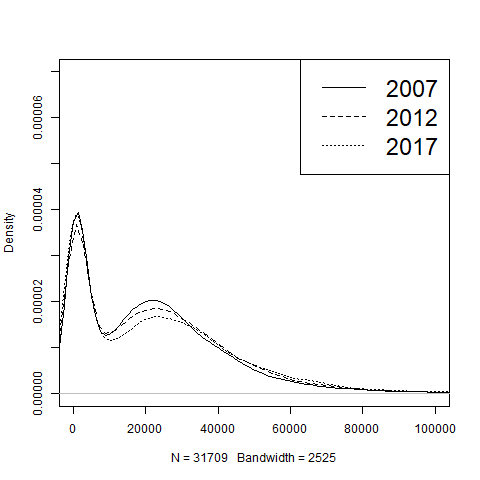
\includegraphics[width=0.60000\textwidth]{img/densityp11.png}
\caption{Pre-tax factor income - Equal sharing}
\end{figure}

\begin{figure}
\centering
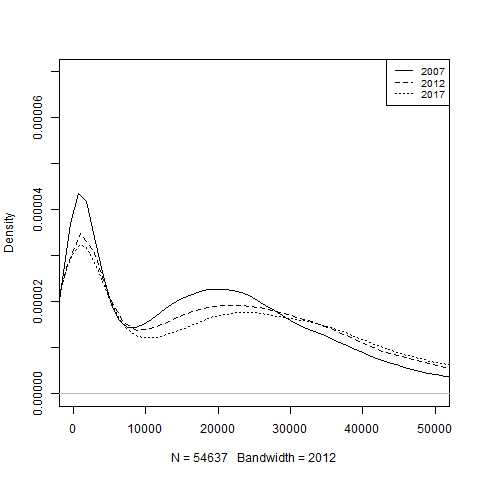
\includegraphics[width=0.60000\textwidth]{img/densityp11closer.png}
\caption{A closer look: Pre-tax factor income - Equal sharing}
\end{figure}

\begin{figure}
\centering
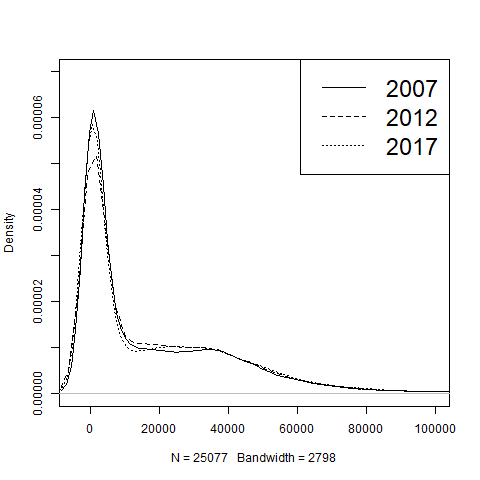
\includegraphics[width=0.60000\textwidth]{img/densityp21.png}
\caption{Pre-tax factor income - Partial sharing}
\end{figure}

\begin{figure}
\centering
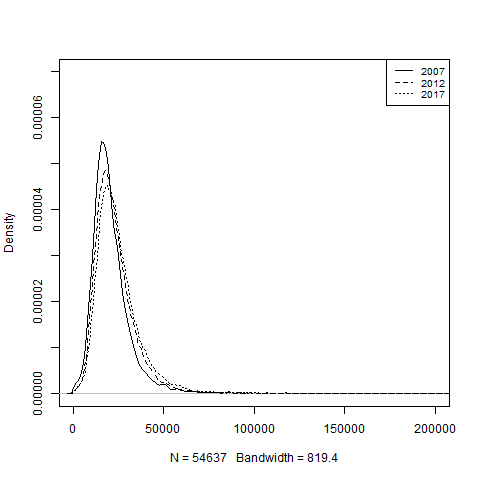
\includegraphics[width=0.60000\textwidth]{img/densityp13.png}
\caption{Post-tax disposable income - Equal sharing}
\end{figure}

\begin{figure}
\centering
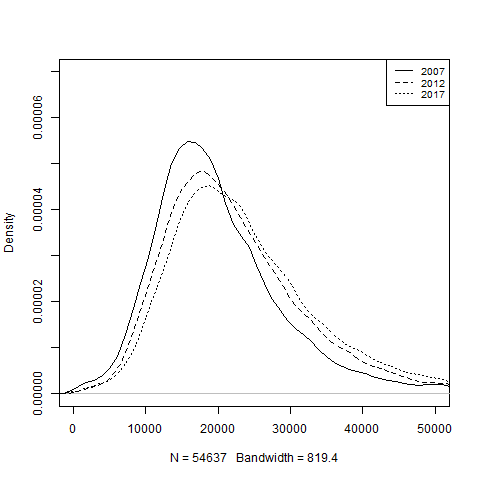
\includegraphics[width=0.60000\textwidth]{img/densityp13closer.png}
\caption{Post-tax disposable income - Equal sharing}
\end{figure}

\begin{figure}
\centering
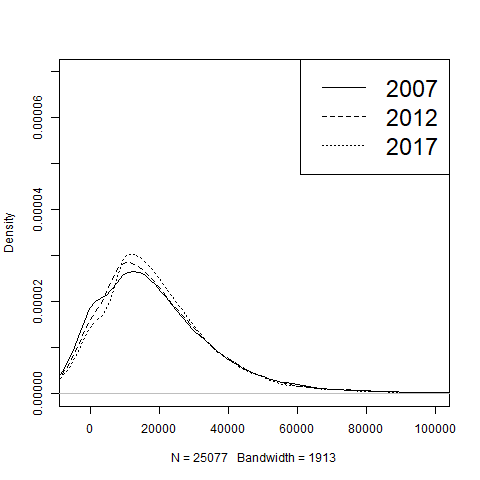
\includegraphics[width=0.60000\textwidth]{img/densityp23.png}
\caption{Post-tax disposable income - Partial sharing}
\end{figure}

\begin{figure}
\centering
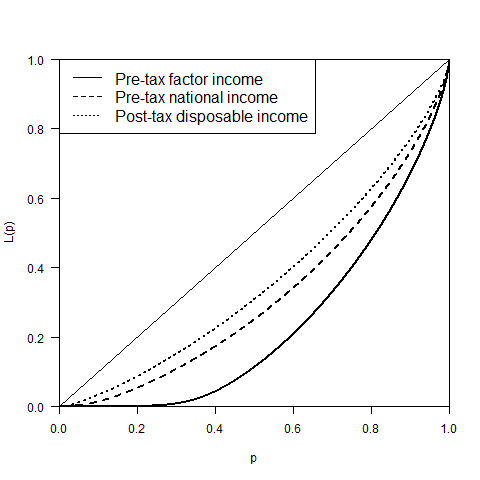
\includegraphics[width=0.60000\textwidth]{img/Lorenzp1.png}
\caption{Lorenz Curve - Equal sharing}
\end{figure}

\begin{figure}
\centering
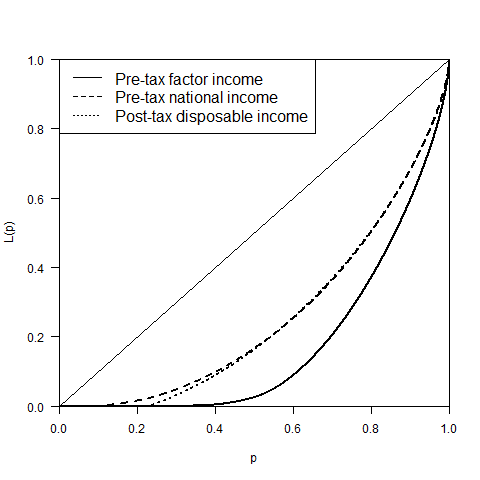
\includegraphics[width=0.60000\textwidth]{img/Lorenzp2.png}
\caption{Lorenz Curve - Partial sharing}
\end{figure}

\section{Tabellen}\label{tabellen}

\begin{longtable}[]{@{}rrrrrr@{}}
\caption{Pre tax factor income - Equal sharing of resources within
household}\tabularnewline
\toprule
Years & Mean & Median & Gini & P80/P20 & Top10\tabularnewline
\midrule
\endfirsthead
\toprule
Years & Mean & Median & Gini & P80/P20 & Top10\tabularnewline
\midrule
\endhead
2005 & 19631 & 17344 & 45.20 & 36.84 & 16.73\tabularnewline
2006 & 17142 & 15023 & 49.34 & 97.92 & 14.76\tabularnewline
2007 & 21922 & 18484 & 50.21 & 96.01 & 27.84\tabularnewline
2008 & 23103 & 19295 & 50.25 & 90.70 & 29.98\tabularnewline
2009 & 22886 & 19395 & 49.51 & 90.04 & 29.41\tabularnewline
2010 & 23204 & 19628 & 49.99 & 98.32 & 31.10\tabularnewline
2011 & 23235 & 19843 & 49.29 & 103.58 & 29.40\tabularnewline
2012 & 24256 & 21054 & 48.28 & 85.68 & 30.72\tabularnewline
2013 & 25131 & 21435 & 49.27 & 91.50 & 34.34\tabularnewline
2014 & 25543 & 22001 & 48.05 & 80.40 & 33.77\tabularnewline
2015 & 26576 & 23094 & 48.14 & 91.05 & 36.15\tabularnewline
2016 & 27570 & 23881 & 47.52 & 80.51 & 38.57\tabularnewline
2017 & 28624 & 24800 & 47.02 & 72.04 & 40.34\tabularnewline
\bottomrule
\end{longtable}

\begin{longtable}[]{@{}rrrrrr@{}}
\caption{Pre tax factor income - Partial sharing of
resources}\tabularnewline
\toprule
Years & Mean & Median & Gini & P80/P20 & Top10\tabularnewline
\midrule
\endfirsthead
\toprule
Years & Mean & Median & Gini & P80/P20 & Top10\tabularnewline
\midrule
\endhead
2005 & 19955 & 15004 & 54.55 & 131.1 & 24.73\tabularnewline
2006 & 16685 & 10003 & 59.54 & 386.1 & 21.84\tabularnewline
2007 & 16943 & 6000 & 65.45 & 861.6 & 33.33\tabularnewline
2008 & 17979 & 6965 & 65.09 & 793.8 & 36.10\tabularnewline
2009 & 17825 & 6865 & 64.37 & 888.8 & 34.85\tabularnewline
2010 & 18207 & 7899 & 63.89 & 990.2 & 35.45\tabularnewline
2011 & 18443 & 8463 & 63.08 & 888.9 & 35.00\tabularnewline
2012 & 19438 & 10000 & 61.88 & 829.0 & 36.15\tabularnewline
2013 & 20677 & 11200 & 61.94 & 933.6 & 39.96\tabularnewline
2014 & 24597 & 18413 & 56.44 & 404.9 & 41.93\tabularnewline
2015 & 25295 & 18646 & 56.86 & 471.4 & 44.19\tabularnewline
2016 & 26230 & 20000 & 55.97 & 477.1 & 45.57\tabularnewline
2017 & 27188 & 21396 & 55.06 & 521.8 & 46.34\tabularnewline
\bottomrule
\end{longtable}

\begin{longtable}[]{@{}rrrrrr@{}}
\caption{Pre tax national income - Equal sharing of resources within
household}\tabularnewline
\toprule
Years & Mean & Median & Gini & P80/P20 & Top10\tabularnewline
\midrule
\endfirsthead
\toprule
Years & Mean & Median & Gini & P80/P20 & Top10\tabularnewline
\midrule
\endhead
2005 & 23796 & 20549 & 32.40 & 5.669 & 14.11\tabularnewline
2006 & 21537 & 18613 & 33.64 & 6.413 & 11.90\tabularnewline
2007 & 26903 & 22403 & 35.93 & 7.085 & 23.15\tabularnewline
2008 & 28311 & 23391 & 36.23 & 7.066 & 25.68\tabularnewline
2009 & 28057 & 23349 & 35.13 & 6.664 & 24.18\tabularnewline
2010 & 28529 & 23693 & 35.95 & 7.067 & 26.08\tabularnewline
2011 & 28392 & 23999 & 35.86 & 7.328 & 25.09\tabularnewline
2012 & 29443 & 25151 & 35.23 & 7.098 & 26.72\tabularnewline
2013 & 30391 & 25500 & 36.20 & 7.335 & 29.40\tabularnewline
2014 & 30536 & 25694 & 35.92 & 7.370 & 29.16\tabularnewline
2015 & 31739 & 27057 & 36.02 & 7.436 & 31.73\tabularnewline
2016 & 32487 & 27742 & 35.92 & 7.320 & 33.18\tabularnewline
2017 & 33644 & 28568 & 35.61 & 7.069 & 35.57\tabularnewline
\bottomrule
\end{longtable}

\begin{longtable}[]{@{}rrrrrr@{}}
\caption{Pre tax national income - Partial sharing of
resources}\tabularnewline
\toprule
Years & Mean & Median & Gini & P80/P20 & Top10\tabularnewline
\midrule
\endfirsthead
\toprule
Years & Mean & Median & Gini & P80/P20 & Top10\tabularnewline
\midrule
\endhead
2005 & 24574 & 20900 & 40.47 & 11.88 & 20.43\tabularnewline
2006 & 21560 & 17953 & 42.47 & 15.18 & 16.84\tabularnewline
2007 & 21089 & 15623 & 52.65 & 92.60 & 27.15\tabularnewline
2008 & 22328 & 16537 & 52.56 & 79.56 & 30.19\tabularnewline
2009 & 22123 & 16794 & 51.55 & 71.32 & 28.42\tabularnewline
2010 & 22677 & 17275 & 51.22 & 61.75 & 29.19\tabularnewline
2011 & 22802 & 17378 & 50.90 & 58.62 & 29.17\tabularnewline
2012 & 23844 & 18307 & 49.87 & 46.06 & 30.57\tabularnewline
2013 & 25249 & 19407 & 49.71 & 40.04 & 33.68\tabularnewline
2014 & 30041 & 24160 & 42.89 & 13.78 & 36.07\tabularnewline
2015 & 30826 & 24500 & 43.31 & 14.03 & 37.64\tabularnewline
2016 & 31510 & 25205 & 42.97 & 13.62 & 38.86\tabularnewline
2017 & 32617 & 26625 & 42.06 & 12.69 & 39.82\tabularnewline
\bottomrule
\end{longtable}

\begin{longtable}[]{@{}rrrrrr@{}}
\caption{Post tax disposable income - Equal sharing of resources within
household}\tabularnewline
\toprule
Years & Mean & Median & Gini & P80/P20 & Top10\tabularnewline
\midrule
\endfirsthead
\toprule
Years & Mean & Median & Gini & P80/P20 & Top10\tabularnewline
\midrule
\endhead
2005 & 18992 & 17009 & 25.04 & 3.496 & 12.69\tabularnewline
2006 & 17807 & 15976 & 25.39 & 3.625 & 10.56\tabularnewline
2007 & 21171 & 18418 & 28.86 & 4.309 & 20.55\tabularnewline
2008 & 22054 & 19147 & 28.99 & 4.306 & 22.89\tabularnewline
2009 & 22039 & 19295 & 28.09 & 4.145 & 22.00\tabularnewline
2010 & 22358 & 19555 & 28.22 & 4.135 & 22.72\tabularnewline
2011 & 22517 & 19900 & 27.78 & 4.083 & 22.24\tabularnewline
2012 & 22907 & 20301 & 27.34 & 4.019 & 23.35\tabularnewline
2013 & 23366 & 20320 & 28.56 & 4.223 & 25.60\tabularnewline
2014 & 23579 & 20582 & 28.54 & 4.256 & 25.88\tabularnewline
2015 & 24483 & 21457 & 28.49 & 4.250 & 28.72\tabularnewline
2016 & 24918 & 22013 & 28.20 & 4.190 & 29.10\tabularnewline
2017 & 25595 & 22616 & 27.91 & 4.111 & 30.89\tabularnewline
\bottomrule
\end{longtable}

\begin{longtable}[]{@{}rrrrrr@{}}
\caption{Post tax disposable income - Partial sharing of
resources}\tabularnewline
\toprule
Years & Mean & Median & Gini & P80/P20 & Top10\tabularnewline
\midrule
\endfirsthead
\toprule
Years & Mean & Median & Gini & P80/P20 & Top10\tabularnewline
\midrule
\endhead
2005 & 20102 & 17176 & 39.34 & 10.445 & 18.77\tabularnewline
2006 & 18154 & 15550 & 39.55 & 10.871 & 15.34\tabularnewline
2007 & 19178 & 14499 & 51.09 & 47.740 & 29.86\tabularnewline
2008 & 20219 & 15342 & 51.14 & 46.681 & 32.56\tabularnewline
2009 & 20078 & 15543 & 50.22 & 45.332 & 31.13\tabularnewline
2010 & 20561 & 15954 & 49.50 & 37.042 & 31.94\tabularnewline
2011 & 20965 & 16469 & 48.53 & 33.912 & 32.15\tabularnewline
2012 & 21719 & 17319 & 47.82 & 30.698 & 33.58\tabularnewline
2013 & 22905 & 17900 & 47.77 & 28.015 & 36.17\tabularnewline
2014 & 23954 & 19379 & 41.15 & 10.690 & 31.74\tabularnewline
2015 & 24559 & 19742 & 41.45 & 10.809 & 33.12\tabularnewline
2016 & 24914 & 20214 & 41.16 & 10.735 & 33.41\tabularnewline
2017 & 25598 & 20993 & 40.19 & 9.979 & 33.50\tabularnewline
\bottomrule
\end{longtable}

\begin{longtable}[]{@{}rrrrrr@{}}
\caption{Post-tax disposable income - Total}\tabularnewline
\toprule
Year & Upper Middle & Middle & Lower Middle & Total Middle & Median
Income\tabularnewline
\midrule
\endfirsthead
\toprule
Year & Upper Middle & Middle & Lower Middle & Total Middle & Median
Income\tabularnewline
\midrule
\endhead
2005 & 16.69 & 56.22 & 15.22 & 88.13 & 17009\tabularnewline
2006 & 19.87 & 55.09 & 12.61 & 87.59 & 15976\tabularnewline
2007 & 14.71 & 52.81 & 17.17 & 84.69 & 18418\tabularnewline
2008 & 14.84 & 52.68 & 17.51 & 85.03 & 19147\tabularnewline
2009 & 15.47 & 53.13 & 16.84 & 85.44 & 19295\tabularnewline
2010 & 15.65 & 52.14 & 17.19 & 84.98 & 19555\tabularnewline
2011 & 16.18 & 52.21 & 16.95 & 85.34 & 19900\tabularnewline
2012 & 16.29 & 52.39 & 16.81 & 85.49 & 20301\tabularnewline
2013 & 16.29 & 51.90 & 16.87 & 85.05 & 20320\tabularnewline
2014 & 15.99 & 51.06 & 16.83 & 83.88 & 20582\tabularnewline
2015 & 15.15 & 51.19 & 17.41 & 83.75 & 21457\tabularnewline
2016 & 14.73 & 50.46 & 18.38 & 83.59 & 22013\tabularnewline
2017 & 14.23 & 51.09 & 18.63 & 83.95 & 22616\tabularnewline
\bottomrule
\end{longtable}

\begin{longtable}[]{@{}rrrrrr@{}}
\caption{Post-tax disposable income - Single Living}\tabularnewline
\toprule
Year & Upper Middle & Middle & Lower Middle & Total Middle & Median
Income\tabularnewline
\midrule
\endfirsthead
\toprule
Year & Upper Middle & Middle & Lower Middle & Total Middle & Median
Income\tabularnewline
\midrule
\endhead
2005 & 15.62 & 49.49 & 15.94 & 81.04 & 17291\tabularnewline
2006 & 20.87 & 45.66 & 12.34 & 78.87 & 17284\tabularnewline
2007 & 16.40 & 45.59 & 13.51 & 75.50 & 18177\tabularnewline
2008 & 15.65 & 46.95 & 13.25 & 75.85 & 18226\tabularnewline
2009 & 17.84 & 47.02 & 12.69 & 77.55 & 18977\tabularnewline
2010 & 16.75 & 43.07 & 14.56 & 74.37 & 18319\tabularnewline
2011 & 16.09 & 44.16 & 14.66 & 74.92 & 18185\tabularnewline
2012 & 15.17 & 44.55 & 14.60 & 74.32 & 18743\tabularnewline
2013 & 15.46 & 44.62 & 14.58 & 74.66 & 19112\tabularnewline
2014 & 14.17 & 44.29 & 15.24 & 73.71 & 19261\tabularnewline
2015 & 15.10 & 44.69 & 13.76 & 73.55 & 20768\tabularnewline
2016 & 14.58 & 45.10 & 15.41 & 75.08 & 21050\tabularnewline
2017 & 13.33 & 45.90 & 15.01 & 74.25 & 21098\tabularnewline
\bottomrule
\end{longtable}

\begin{longtable}[]{@{}rrrrrr@{}}
\caption{Post-tax disposable income - Two Children}\tabularnewline
\toprule
Year & Upper Middle & Middle & Lower Middle & Total Middle & Median
Income\tabularnewline
\midrule
\endfirsthead
\toprule
Year & Upper Middle & Middle & Lower Middle & Total Middle & Median
Income\tabularnewline
\midrule
\endhead
2005 & 13.57 & 60.78 & 15.61 & 89.96 & 15803\tabularnewline
2006 & 16.30 & 62.31 & 11.41 & 90.07 & 15229\tabularnewline
2007 & 12.45 & 58.25 & 16.32 & 87.03 & 18620\tabularnewline
2008 & 11.36 & 58.35 & 17.81 & 87.52 & 19408\tabularnewline
2009 & 13.31 & 58.10 & 16.65 & 88.06 & 19905\tabularnewline
2010 & 14.08 & 57.91 & 16.17 & 88.16 & 20300\tabularnewline
2011 & 14.44 & 57.35 & 16.63 & 88.42 & 20373\tabularnewline
2012 & 14.62 & 57.02 & 16.51 & 88.16 & 20912\tabularnewline
2013 & 15.71 & 56.40 & 16.11 & 88.22 & 21017\tabularnewline
2014 & 12.89 & 57.48 & 15.92 & 86.29 & 20185\tabularnewline
2015 & 11.22 & 56.77 & 19.39 & 87.38 & 20997\tabularnewline
2016 & 10.68 & 54.84 & 20.34 & 85.86 & 21461\tabularnewline
2017 & 10.75 & 57.91 & 18.88 & 87.54 & 22352\tabularnewline
\bottomrule
\end{longtable}

\begin{longtable}[]{@{}rrrrrr@{}}
\caption{Post-tax disposable income - Older}\tabularnewline
\toprule
Year & Upper Middle & Middle & Lower Middle & Total Middle & Median
Income\tabularnewline
\midrule
\endfirsthead
\toprule
Year & Upper Middle & Middle & Lower Middle & Total Middle & Median
Income\tabularnewline
\midrule
\endhead
2005 & 14.469 & 56.70 & 16.52 & 87.69 & 16833\tabularnewline
2006 & 15.672 & 56.72 & 15.57 & 87.97 & 15270\tabularnewline
2007 & 10.908 & 51.35 & 23.49 & 85.75 & 16414\tabularnewline
2008 & 11.117 & 52.50 & 23.25 & 86.86 & 17255\tabularnewline
2009 & 11.459 & 53.33 & 22.49 & 87.27 & 17604\tabularnewline
2010 & 12.036 & 52.86 & 22.68 & 87.57 & 17719\tabularnewline
2011 & 12.771 & 53.64 & 21.17 & 87.58 & 18263\tabularnewline
2012 & 12.696 & 53.09 & 21.77 & 87.55 & 18479\tabularnewline
2013 & 12.956 & 52.85 & 21.60 & 87.41 & 18771\tabularnewline
2014 & 13.019 & 50.90 & 21.78 & 85.70 & 19032\tabularnewline
2015 & 10.448 & 51.15 & 23.79 & 85.38 & 19524\tabularnewline
2016 & 9.055 & 50.50 & 24.89 & 84.45 & 19757\tabularnewline
2017 & 9.845 & 50.61 & 25.26 & 85.72 & 20235\tabularnewline
\bottomrule
\end{longtable}

\hypertarget{refs}{}
\hypertarget{ref-grabka2016schrumpfender}{}
Grabka, Markus M, Jan Goebel, Carsten Schröder, and Jürgen Schupp. 2016.
``Schrumpfender Anteil an Bezieherinnen Mittlerer Einkommen in Den Usa
Und Deutschland.'' \emph{DIW-Wochenbericht} 83 (18). Berlin: Deutsches
Institut für Wirtschaftsforschung (DIW): 391--402.

\hypertarget{ref-niehues2017mittelschicht}{}
Niehues, Judith. 2017. ``Die Mittelschicht in Deutschland: Vielschichtig
Und Stabil.'' \emph{IW-Trends--Vierteljahresschrift Zur Empirischen
Wirtschaftsforschung} 44 (1). Köln: Institut der deutschen Wirtschaft
Köln (IW): 3--20.

\hypertarget{ref-niehues2013arm}{}
Niehues, Judith, Thilo Schaefer, and Christoph Schröder. 2013. ``Arm Und
Reich in Deutschland: Wo Bleibt Die Mitte.'' \emph{Definition, Mythen
Und Fakten. Köln: Inst. Der Dt. Wirtschaft}.


\end{document}
